\documentclass{article}
\pdfpagewidth=8.5in
\pdfpageheight=11in


\usepackage{ijcai23}
\usepackage{times}
\usepackage{soul}
\usepackage{url}
\usepackage[hidelinks]{hyperref}
\usepackage[utf8]{inputenc}
\usepackage[small]{caption}
\usepackage{graphicx}
\usepackage{amsmath}
\usepackage{amsthm}
\usepackage{booktabs}
\usepackage{algorithm}
\usepackage{algorithmic}
%\usepackage[switch]{lineno}

\urlstyle{same}

\newtheorem{example}{Example}
\newtheorem{theorem}{Theorem}

\pdfinfo{
/RelatórioFinal
}


\title{Database-driven Chatbot}


% Single author syntax
\author{
    Eduardo Neves
    \affiliations
    Universidade de Coimbra
    \emails
    eduardofbneves@gmail.com
}


\begin{document}

\maketitle

\begin{abstract}
No panorama atual, vê-se em várias plataformas algoritmos de comunicação com pessoas. Presentes muitas aplicações, estes podem ser encontrados em vários \textit{websites} banais. A sua utilidade no mundo empresarial viu até crescer mecanismos de construção personalizada de \textit{Chatbots}. Neste trabalho planeia-se desenvolver os mecanismos para a construção de um \textit{Chatbot AI} com recurso a \textit{Machine Learning}.
\end{abstract}

\section{Introdução}
Uma \textit{Conversational AI} é um algoritmo de Inteligência Artificial que simula conversação humana com implementação em vários meios. Há dois tipos de \textit{Chatbots}: de domínio fechado, que responde com mensagens pré-definidas e generativos, que geram as respostas consoante o \textit{input}. Com \textit{Machine Learning} (ML) o modelo aprende com dados de um conjunto. Um conceito comum neste campo é o de processamento de linguagem natural (NLP em inglês) que se preocupa com a interação entre humanos e máquinas. 


\section{Dados e Abordagem}
Os dados para um \textit{Chatbot} baseiam-se principalmente em sequências de interações entre partes. Os \textit{datasets} podem variar entre pergunta e resposta, a e-mails trocados ou conversas em plataformas online entre indivíduos. Para este trabalho foi usado um conjunto de dados baseado em em legendas de filmes para português.

\subsection{Conjunto de dados}
O pacote de dados usado foi tirado do projeto "OPUS ... the open parallel corpus" \cite{opus}, um 'corpus' de textos traduzidos da Internet baseada em produtos 'open source'. O \textit{dataset} utilizado é atualmente distribuído pela plataforma "opensubtitles" \cite{opensubtitles}, de onde foi retirado o conteúdo.

Como o foco do projeto é um algoritmo em português, retirou-se o \textit{dataset} "pt" \cite{lison-tiedemann-2016-opensubtitles2016}, que coleciona mais de 40000 ficheiros de legendas de filmes até o ano de 2017. Separados por anos, alguns filmes contam com várias versões do mesmo filme. O seu tratamento é explicado na secção seguinte. 

\subsection{Tratamento dos dados}
Com o conjunto de dados inicial com redundâncias e pouco estruturado, procurou-se correr um pequena organização à informação. A preparação da entrada para treino é feita aquando a inicialização do processo. Esta encontra-se no \textit{script} "train.py".

\subsubsection{Redução de redundâncias}
Como referido, algumas versões do mesmo filme são dispostas e organizadas em conjunto. Ao remover este entrave, pode-se retirar uma camada na diretoria e agrupar apenas por ano. Apesar desta diferenciação não ser necessária poderá ser útil em comparações ortográficas ou até numa maior confiança de traduções mais recentes. Para selecionar o ficheiro mais relevante apenas se selecionou o ficheiro com menor volume de espaço no disco para melhor \textit{performance}.

\subsubsection{Alteração do formato}
O \textit{dataset} original continha apenas ficheiros em .xml, com muitos elementos, como tempos e personagens, desnecessárias a este trabalho. Outra especificação sem relevância é a separação por palavras das falas de cada personagem. Simplificou-se então para um formato .json, onde cada entrada é a fala de uma personagem. Manteve-se a separação dos ficheiros por filmes.

\begin{figure}
	\centering
    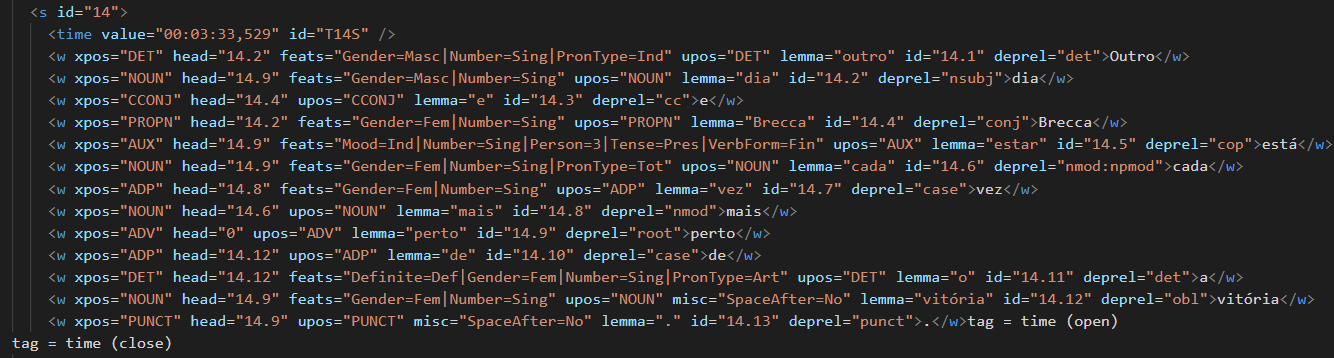
\includegraphics[scale=0.3]{xml.png}
    \caption{Formato original do \textit{dataset} para um filme aleatório}
    \label{xmlimg}
\end{figure}

\begin{figure}
	\centering
    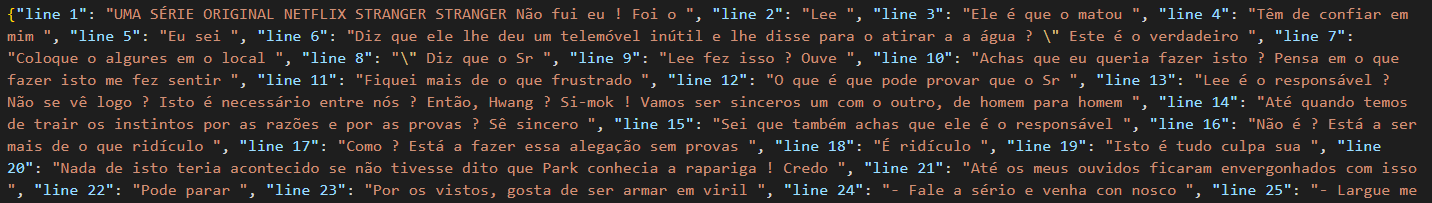
\includegraphics[scale=0.28]{json.png}
    \caption{Formato alterado de um filme aleatório do conjunto}
    \label{jsonimg}
\end{figure}

\subsubsection{Redução de amostragem}
Para além da redução na alteração do formato, reduziu-se também a quantidade de dados usados para o programa. Utilizou-se apenas filmes a partir de 2000, o que resultou em 37851 filmes, com uma média de 455 falas de personagens, condensados em cerca de $1.2$GB. Este ainda assim é um número muito grande de filmes, mas manteve-se para manutenção da utilidade do conjunto, além de uma maior escolha entre filmes de vários anos para possível teste.

\subsubsection{Preparação para treino}
Na língua portuguesa deparamo-nos com vários acentos e outros símbolos como os traços (como exemplo "ensino-te"). Quanto aos acentos, a sua manutenção é imperativa para boa leitura e para remoção de confusões entre palavras (como por exemplo "estás" e "estas"). Por outro lado, os traços foram retirados("ensino-te" para "ensino" " te"), já que a flexão do pronomes quanto ao número e género é demasiado vasta para garantir um vocabulário conciso e para boa predição do modelo. Outros símbolos de sintaxe e gramaticais foram retirados aquando a preparação para treino.


\subsection{Modelo}


\subsubsection{LSTM}
A 'Long Short Term Memory' (LSTM) é uma rede neuronal recorrente capaz de aprender a dependência em problemas de predição. Esta é útil em tradução, reconhecimento de fala e, direcionado para este tópico, simulação de conversação humana. Mais sobre este tipo de redes, elas têm um estado interno que consegue representar informação em contexto \cite{bengio1994learning}.

\subsubsection{Seq2seq}
A metodologia 'sequence-to-sequence' (seq2seq) é a peça-chave do trabalho. A metodologia utiliza modelos de 'Machine Learning' (ML) para obter um sequência como entrada, num domínio, e convertê-la para uma representação noutro domínio. 

O \textit{seq2seq} baseia-se num bloco \textit{encoder} que lê a série de entrada a partir de um vetor de dimensionalidade fixa e um bloco \textit{decoder} que extrai a frase. Ambos estes blocos são células LSTM e são treinados ao mesmo tempo \cite{sutskever2014sequence}. Entre eles há um vetor de contexto que encapsula todo o sentido da frase.

\begin{figure}[h]
    \centering
    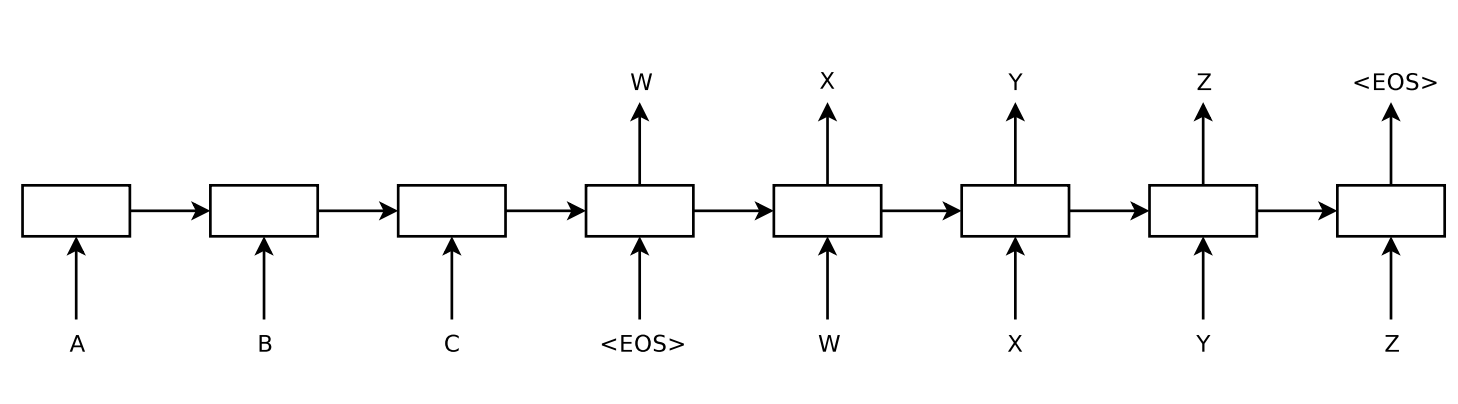
\includegraphics[scale=0.3]{encoder_decoder.png}
    \caption{Ilustração da metodologia. os primeiros quatro retêngulos referem-se à camada \textit{encoder} enquanto o resto pertence à \textit{decoder}}
    \cite{sutskever2014sequence}
    \label{fig1}
\end{figure}


No momento inicial, quando é fornecida uma sequência ao modelo, a frase terá de caber no vetor fixo, portanto leva \textit{padding}. À sequência acrescentam-se componentes "\textless PAD\textgreater ". Ao passar pelo vetor, o \textit{decoder} inicia com o comando "\textless START\textgreater ", ou "\textless GO\textgreater " como usado neste trabalho, para iniciar a produção da saída. A sequência é completa com a expressão "\textless EOS\textgreater " que simboliza o final do \textit{output}. Para expressões que o algoritmo não reconhece lança-se o comando "\textless UNK\textgreater ".

Para além destas, estes modelos contemplam ainda duas camadas de 'embedding', para cada um dos blocos referidos. Esta reduz a dimensão dos vetores de entrada e representam melhor estas sequências \cite{li2018slim}. 

\subsubsection{'Attention'}
Em ML, esta técnica tem o objetivo de reproduzir atenção cognitiva (comportamento humano). O efeito traduz-se em realçar algumas partes da entrada, enquanto diminui outras, mudando o foco da informação dada. Este método é também sensível ao contexto, algo que é tido em conta no treino da máquina. 

\subsection{Código utilizado}
O modelo base foi retirado da plataforma Github, do repositório Seq2Seq-Chatbot \cite{abonia2020seq2seq}. Este modelo usa o módulo \textit{tensorflow} para os processos de ML.

No trabalho citado foi também usado um \textit{dataset} de filmes, o 'Cornell Movie Dialog Corpus' \cite{cornell}. Este dispunha de 304713 entradas para treino num ficheiro .txt também disponibilizado.

\begin{table}[htb]
    \centering
    \begin{tabular}{l | l l}
        \hline
        Parâmetros  & Config1 & Config2 \\
        \hline
        'batch size' &  128  &  512 \\
        tamanho 'embedding' &  128     &  512  \\
        tamanho RNN  & 128     &  512 \\
        'epochs' &  500  &  100 \\
    \end{tabular}
    \caption{Excerto da tabela fornecida pela autora}
    \cite{sojasingarayar2020seq2seq}
    \label{tabmodel}
\end{table}

Seguiu-se com a configuração 1 para estre trabalho onde a autora conseguiu valores de exatidão na ordem dos $62\%$ e de perda de $19\%$ \cite{sojasingarayar2020seq2seq}.

\begin{figure}[htb]
    \centering
    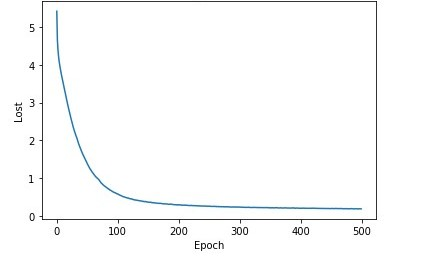
\includegraphics[scale=0.8]{abonialoss}
    \caption{Gráfico fornecido pela autora e pretendido para o trabalho}
    \label{abonialoss}
\end{figure}

Na abordagem para este trabalho, pegou-se no \textit{script} de 'Python' referente ao modelo na íntegra. O restante código foi construído para executar o modelo, à semelhança do produto original.

\section{Experimentação e Métricas}
\label{metricas}
\subsection{BLEU}
'Bilingual Evaluation Understudy Score' (BLEU) compara a sequência de resposta com a ideal. A métrica compara os conjuntos de caracteres, independentemente da ordem. O BLEU conta as \textit{n-grams} e conta o número de coincidências \cite{papineni2002bleu}. Este método é maioritariamente para algoritmos de tradução de texto portanto, para este trabalho, as pontuações esperadas não são muito elevadas. 

\subsection{ROUGE}
'Recall-Oriented Understudy for Gisting Evaluation' é um conjunto de métricas especializadas em avaliar \textit{machine translation}. Estas métricas focam-se em quanto as palavras (ou \textit{n-grams} no input se assemelham às previstas pelo modelo.

Neste trabalho foca-se no ROUGE-L que se baseia na subsequência mais longa em comum entre o \textit{output} e a referência. Uma vantagem do uso desta métrica é que não é necessário ter correspondências consecutivas, mas correspondências em sequência \cite{rouge}. A implementação é feita com recurso ao módulo "rouge" do \textit{python}.

\subsection{\textit{f1-score}}
Com os valores anteriores consegue-se computar o \textit{f1-score}. Este define-se pela média de precisão e do \textit{recall}. Diferencia-se a média, usando-se a média harmónica e não a aritmética.

\begin{equation}
F1 = \frac{2*BLEU*ROUGE}{BLEU+ROUGE}
\end{equation}


\section{Resultados}

Partindo das especificações da autora na Tabela \ref{tabmodel}, rapidamente se chegou à conclusão que estes parâmetros requeria muito esforço computacional. Desta forma conduziram-se vários testes ao variar as \textbf{\textit{epochs}} e a \textbf{quantidade de filmes} para treinar o modelo.
\subsection{Treino}
Para o treino seguiram-se os parâmetros da referência \cite{abonia2020seq2seq} e um tamanho de dados de treino semelhante. No entanto o treino demorava mais de 20 horas a correr tudo. Desta forma fizeram-se vários testes para tentar encontrar um valor ideal de \textit{epochs} que reproduzisse resultados fiáveis sem requerer de demasiado poder computacional.

\subsubsection{Para 85 e 100 \textit{epochs}}
\begin{figure}[htb]
    \centering
    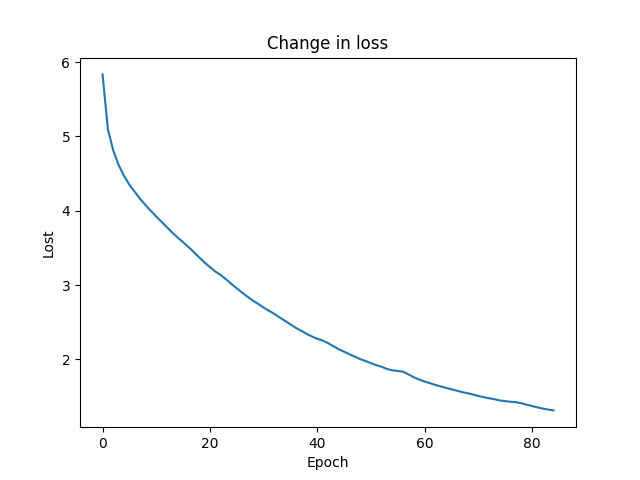
\includegraphics[scale=0.35]{85loss}
    \caption{}
    \label{85loss}
\end{figure}
\begin{figure}[htb]
    \centering
    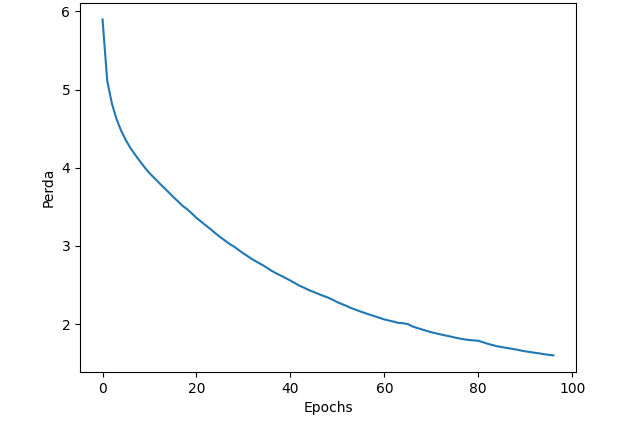
\includegraphics[scale=0.35]{100epochs}
    \caption{Gráficos de variação da perda consoante as \textit{epochs}}
    \label{100loss}
\end{figure}
Estes valores foram tentados segundo o gráfico mostrado na figura \ref{abonialoss}. Ambas as tentativas utilizaram 500 filmes e duraram acima de 8 horas cada.

Em ambas as tentativas, a perda não baixou do valor 1, o que revela poucas iterações de treino. No entanto a curva, perto dos valores máximos, está a tender para um valor constante. Com estes testes foi possível também inferir que, para treinos com um maior número de dados a perda inicial é maior.

\subsubsection{150 \textit{epochs}}
\begin{figure}[h]
    \centering
    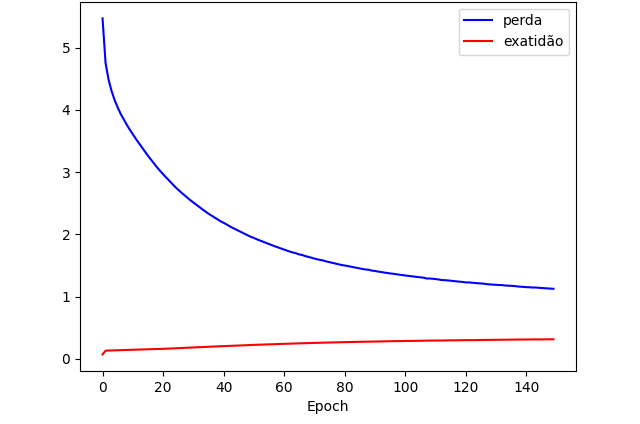
\includegraphics[scale=0.4]{150epochs1000movies}
    \caption{Gráficos de variação da perda consoante as \textit{epochs}}
    \label{150epochs}
\end{figure}

Para este treino foram usados 1000 filmes, para entender como poderia variar o desempenho do modelo consoante o tamanho da amostra. Verificou-se que este aumento afeta principalmente o vocabulário aprendido pela máquina, mas apesar de tudo a 'performance' não melhora significativamente.

\subsection{Teste}

Para os testes retiraram-se filmes aleatórios da base de dados para retirar valores dos testes mencionados na secção \ref{metricas}. Para tamanho dos dados de teste usou-se $30\%$ dos dados de treino $(70-30)$.\\

Os valores médios obtidos para as métricas foram os seguintes:
$$ BLEU = 1.3769041687735495e-231$$
$$ ROUGE = 0.033094944870102116$$
Retirou-se então um valor de BLEU muito perto de 0. Desta forma, o \textit{f1-score} irá ser também 0 virtualmente. Estes valores, apesar de se esperar um valor baixo, tendo em conta que se trata de um \textit{chatbot}. No entanto estes são valores impensáveis para um modelo de qualidade. Por estes valores podemos concluir que o modelo é desatualizado ou o treino do modelo não foi o adequado.

\subsection{'Chat'}
Em algumas conversas com o algoritmo, reparou-se nalguns padrões, como o foco em palavras específicas e repetição da expressão perante várias entradas diferentes. Este problema é mais grave quando uma das palavras é um nome ou uma expressão estrangeira. 
\begin{figure}[h]
    \centering
    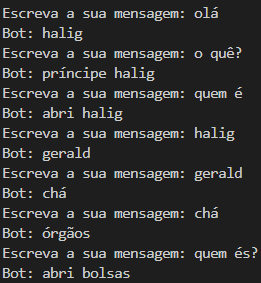
\includegraphics[scale=0.7]{exemplo_chat.png}
    \caption{Exemplo da repetição da palavra "halig", que nem pertence ao dicionário português segundo o dicionário "priberam"}
    \label{chat1}
\end{figure}
\begin{figure}[h]
    \centering
    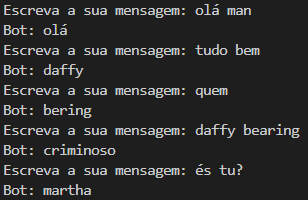
\includegraphics[scale=0.7]{chat1}
    \caption{Outra situação de fixação de nomes, que são mencionados sem qualquer contexto}
    \label{chat2}
\end{figure}

No entanto, alguns treinos com iterações mais elevadas (perto dos 200 \textit{epochs} revelaram algumas conversas com respostas com algum sentido, mas sem contexto na conversa que se seguia.
\begin{figure}[htb]
    \centering
    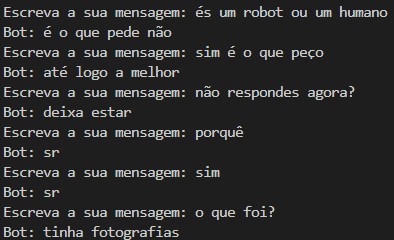
\includegraphics[scale=0.7]{chat2}
    \caption{o modelo também dispersa facilmente}
    \label{chat3}
\end{figure}

O \textit{chatbot} responde aos mesmos inputs de forma diferente consoante a conversa avança. Este efeito era esperado, pelo que afere-se que o modelo é sensível ao desenrolar da conversa e do contexto que é dado.

\section{Problemas e Possíveis Resoluções}

\subsection{Conjunto de dados}
Alguns problemas foram encontrados no uso da informação.

Em primeiro lugar, muitos ficheiros continham referências aos tradutores como parte das legendas. Como estas variavam em formato e local era difícil prever e retirar estas informações com sucesso.

Algumas traduções eram também desvirtuadas do português Portugal, tais como o uso de expressões como "em a", em vez de "na" em vários locais. A fonte oferecia também um pacote de português Brasil, portanto estas nuances não se esperariam no conjunto usado. Pequenas alterações como esta seriam de difícil execução sem uma análise extensiva dos dados.

\subsubsection{Resolução}
A melhor resolução seria uma pesquisa e análise extensiva de todo o \textit{dataset} para remoção de erros e para escolha dos melhores ficheiros a utilizar. Isto seria algo pouco exequível num conjunto daquela dimensão, onde certamente se iriam descartar várias informações. Outro solução seria a alteração de algumas sequências de caracteres por outras mais enquadradas com a língua. A substituição poderia acarretar vários erros já que se iria analisar sequências que poderiam não estar isoladas de outras para formar palavras. Ao abrir alguns ficheiros .json, verificou-se que alguns deles possuíam poucas linhas de texto, na ordem das 30 ou 40, o que se afasta muito da média de linhas por ficheiro que ronda as 450. Visto que se escolheu um tamanho de treino de ficheiros limitado, estes tornam-se \textit{outliers} no panorâma maior do \textit{dataset} e podem influenciar na execução do treino. 

Apesar destes problemas, usou-se este 'dataset' pela sua vastidão e facilidade de acesso. Acrescendo a dificuldade de materiais para a língua desejada, esta foi a melhor opção encontrada.

\subsection{Modelo}
A escolha do código foi influenciada na metodologia seq2seq (aconselhada pelo professor). A pesquisa foi então restringida para tal.

O uso desta versão 1.14 do \textit{tensorflow} é desatualizada, pois o pacote está já na versão 2 a partir de 2019. Esta veio com uma mudança na organização e, portanto, na sintaxe a usar para construir o modelo. Obriga, também, ao uso de uma versão anterior do python (3.6 ou menor). 

Este modelo traz então algumas agravantes, em especial o tempo de compilação. Para 500 filmes com 100 \textit{epochs}, o tempo tomado foi cerca de 10 horas todo o processo de treino. Com estes números o modelo leva a um esforço computacional aquém do esperado, tornando-se até inexequível em termos de desenvolvimento do trabalho.

\subsubsection{Resoluções}

Melhores resultados poderiam ser obtidos com maior poder computacional. Apesar das falhas do \textit{dataset}, considerou-se suficiente para obter resultados razoáveis. 

Para melhoria de execução, e até suporte, alterações do código para suportar a versão 2 do \textit{tensorflow} poderiam ser executadas. Para manutenção do modelo da autora, esta alteração não foi feita, mas seria proveitosa para a execução do trabalho.

\section{Conclusões}
Em suma, considera-se que o produto final não corresponde às expectativas e não consegue encetar numa conversa normal com algum nexo. Esta conclusão, apesar de evidente quando se executa uma conversa, foi confirmado pelas métricas do relatório.

Por outro lado, o modelo mostrou progressão e mostra indícios de produzir conversas com algum sentido, apesar de esta ser uma métrica mais volátil e subjetiva. Acrescenta-se o facto de o procedimento recomendado não ter sido seguido à risca, pelos motivos mencionados. Possivelmente, ao seguir estas indicações, os resultados seriam proveitosos. Em última análise concluo que o trabalho de pesquisa e de evolução deste modelo resultou num projeto conjunto com alguma qualidade.


\bibliographystyle{named}
\bibliography{biblio.bib}

\end{document}

